\section{Word Representation}

The general idea behind word representation is to convert the text into an understandable format for the computer. This is done by word embedding which learns a vector representation for words.

\subsection{Types of embeddings} \label{types_embeddings}

There are several different approaches used for encoding words: 

\begin{enumerate}
    \item \textbf{Bag-of-Words (BOW):} The simplest approach for word encoding is the Bag-Of-Words approach where the general concept is to generate a dictionary of tokens from the text (say, news articles) by pre-processing the text using techniques such as stopword removal, lemmatisation and Named Entity Detection (NER) and then represent the documents/ news articles as a vector of the occurrences of those tokens in the text. In other words, the $j_{th}$ element in the vector (say 5) represents the fact that the $j_{th}$ token in the dictionary (say `London') appeared 5 times. This method is fairly primitive as it does not account for any grammatical rules and is an unordered representation. It falls short with increasingly high volumes of data as it is simply a syntactic representation and does not account for any semantic/ conceptual relations within the text corpus~\cite{elmo_word_rep}.
    

    \item \textbf{Term-Frequency-Inverse Document Frequency (TF-IDF):}  TF-IDF is a numerical statistic that indicates the significance of a word in a corpus (collection of documents). It is frequently used as a weighting factor in conjunction with the bag-of-words approach to represent document embeddings. The TF-IDF value is proportional to term frequency (TF) which represents the number of times a word appears in the document and is countered by the number of documents in the corpus that contain this word (IDF), thereby compensating for the fact that some words appear more frequently in general, and their high frequency is not distinct to a document~\cite{tfidf_mining}.
    
    \item \textbf{Word2Vec:} Word2Vec algorithms provide a much better way of word representation (or embedding) by using the concept of similarity of words. The core idea is that words that are syntactically and semantically close should have similar vector representations and thereby occupy similar spatial positions. This degree of similarity is calculated using the cosine similarity (cosine of the angle between two vectors)~\cite{efficient_word_rep}. They also exploit the `locality hypothesis' which centres around the notion that words that appear together or are close to identical  will be spatially close~\cite{elmo_word_rep}.

For simplicity's sake, let's say the word `know' is represented by a 4-dimensional binary vector [\_,\_,1,\_], with 1 in the third dimension then vectors for words that are variants of the same underlying root word such as `knew', `known' etc. will also have 1 in the third dimension, and those are not (say, `Monday') will not. Similarly, there can be a feature (dimension) (say, the $4_{th}$ dimension) representing a word type or category such as airlines and so, for instance, `Emirates', `Etihad' and `British Airways' should also have similar vector representations with the $4_{th}$ dimension (feature) having a value of 1, thereby assigning them to the same group (cluster)~\cite{32_contextual_word}.

These Word2Vec embeddings are commonly used in the Neural Network models: Continuous Skip-Gram and Continuous Bag-of-Words (CBoW)~\cite{efficient_word_rep}.

\item \textbf{GloVe:} Another popular approach is using GloVe or Global Vectors for word representation. Unlike word2vec which leverages co-occurrence of neighbouring words within local context, the GloVe unsupervised model focuses on global statistics of word co-occurrences over the whole corpus. Like word2vec, it also relies on the mapping words in vector subspaces using semantic similarity of words \cite{glove}. 

\item \textbf{Context2Vec:} An improvement over Word2Vec is Context2Vec. This accounts for polysemy, the fact that in different contexts, words can have different meanings (or senses). This allows for a context-independent representation for a word, called
``contextual word vectors" which encapsulate the meaning for a word in a particular context. For instance, in the context of the sentence ``I ate a banana split", `split', is associated with food~\cite{32_contextual_word} and in ``the ice cracked and split'', `split' is a verb indicating breakage of ice.

This approach makes use of a bi-directional (left-to-right and right-to-left) LSTM (long short-term memory) recurring neural network. This network makes use of N layers of LSTM, where the lower levels extract low-level features such as POS tagging and the upper levels learn the contextual meaning of words ~\cite{elmo_word_rep}. One of the most popular approaches for this is ELMo (Embeddings from Language Models) which is discussed in \Cref{elmo}.
\end{enumerate}

\subsection{Embeddings from Language Models (ELMo)} \label{elmo}
\vspace{-4ex}

\begin{figure}[H]
\centering
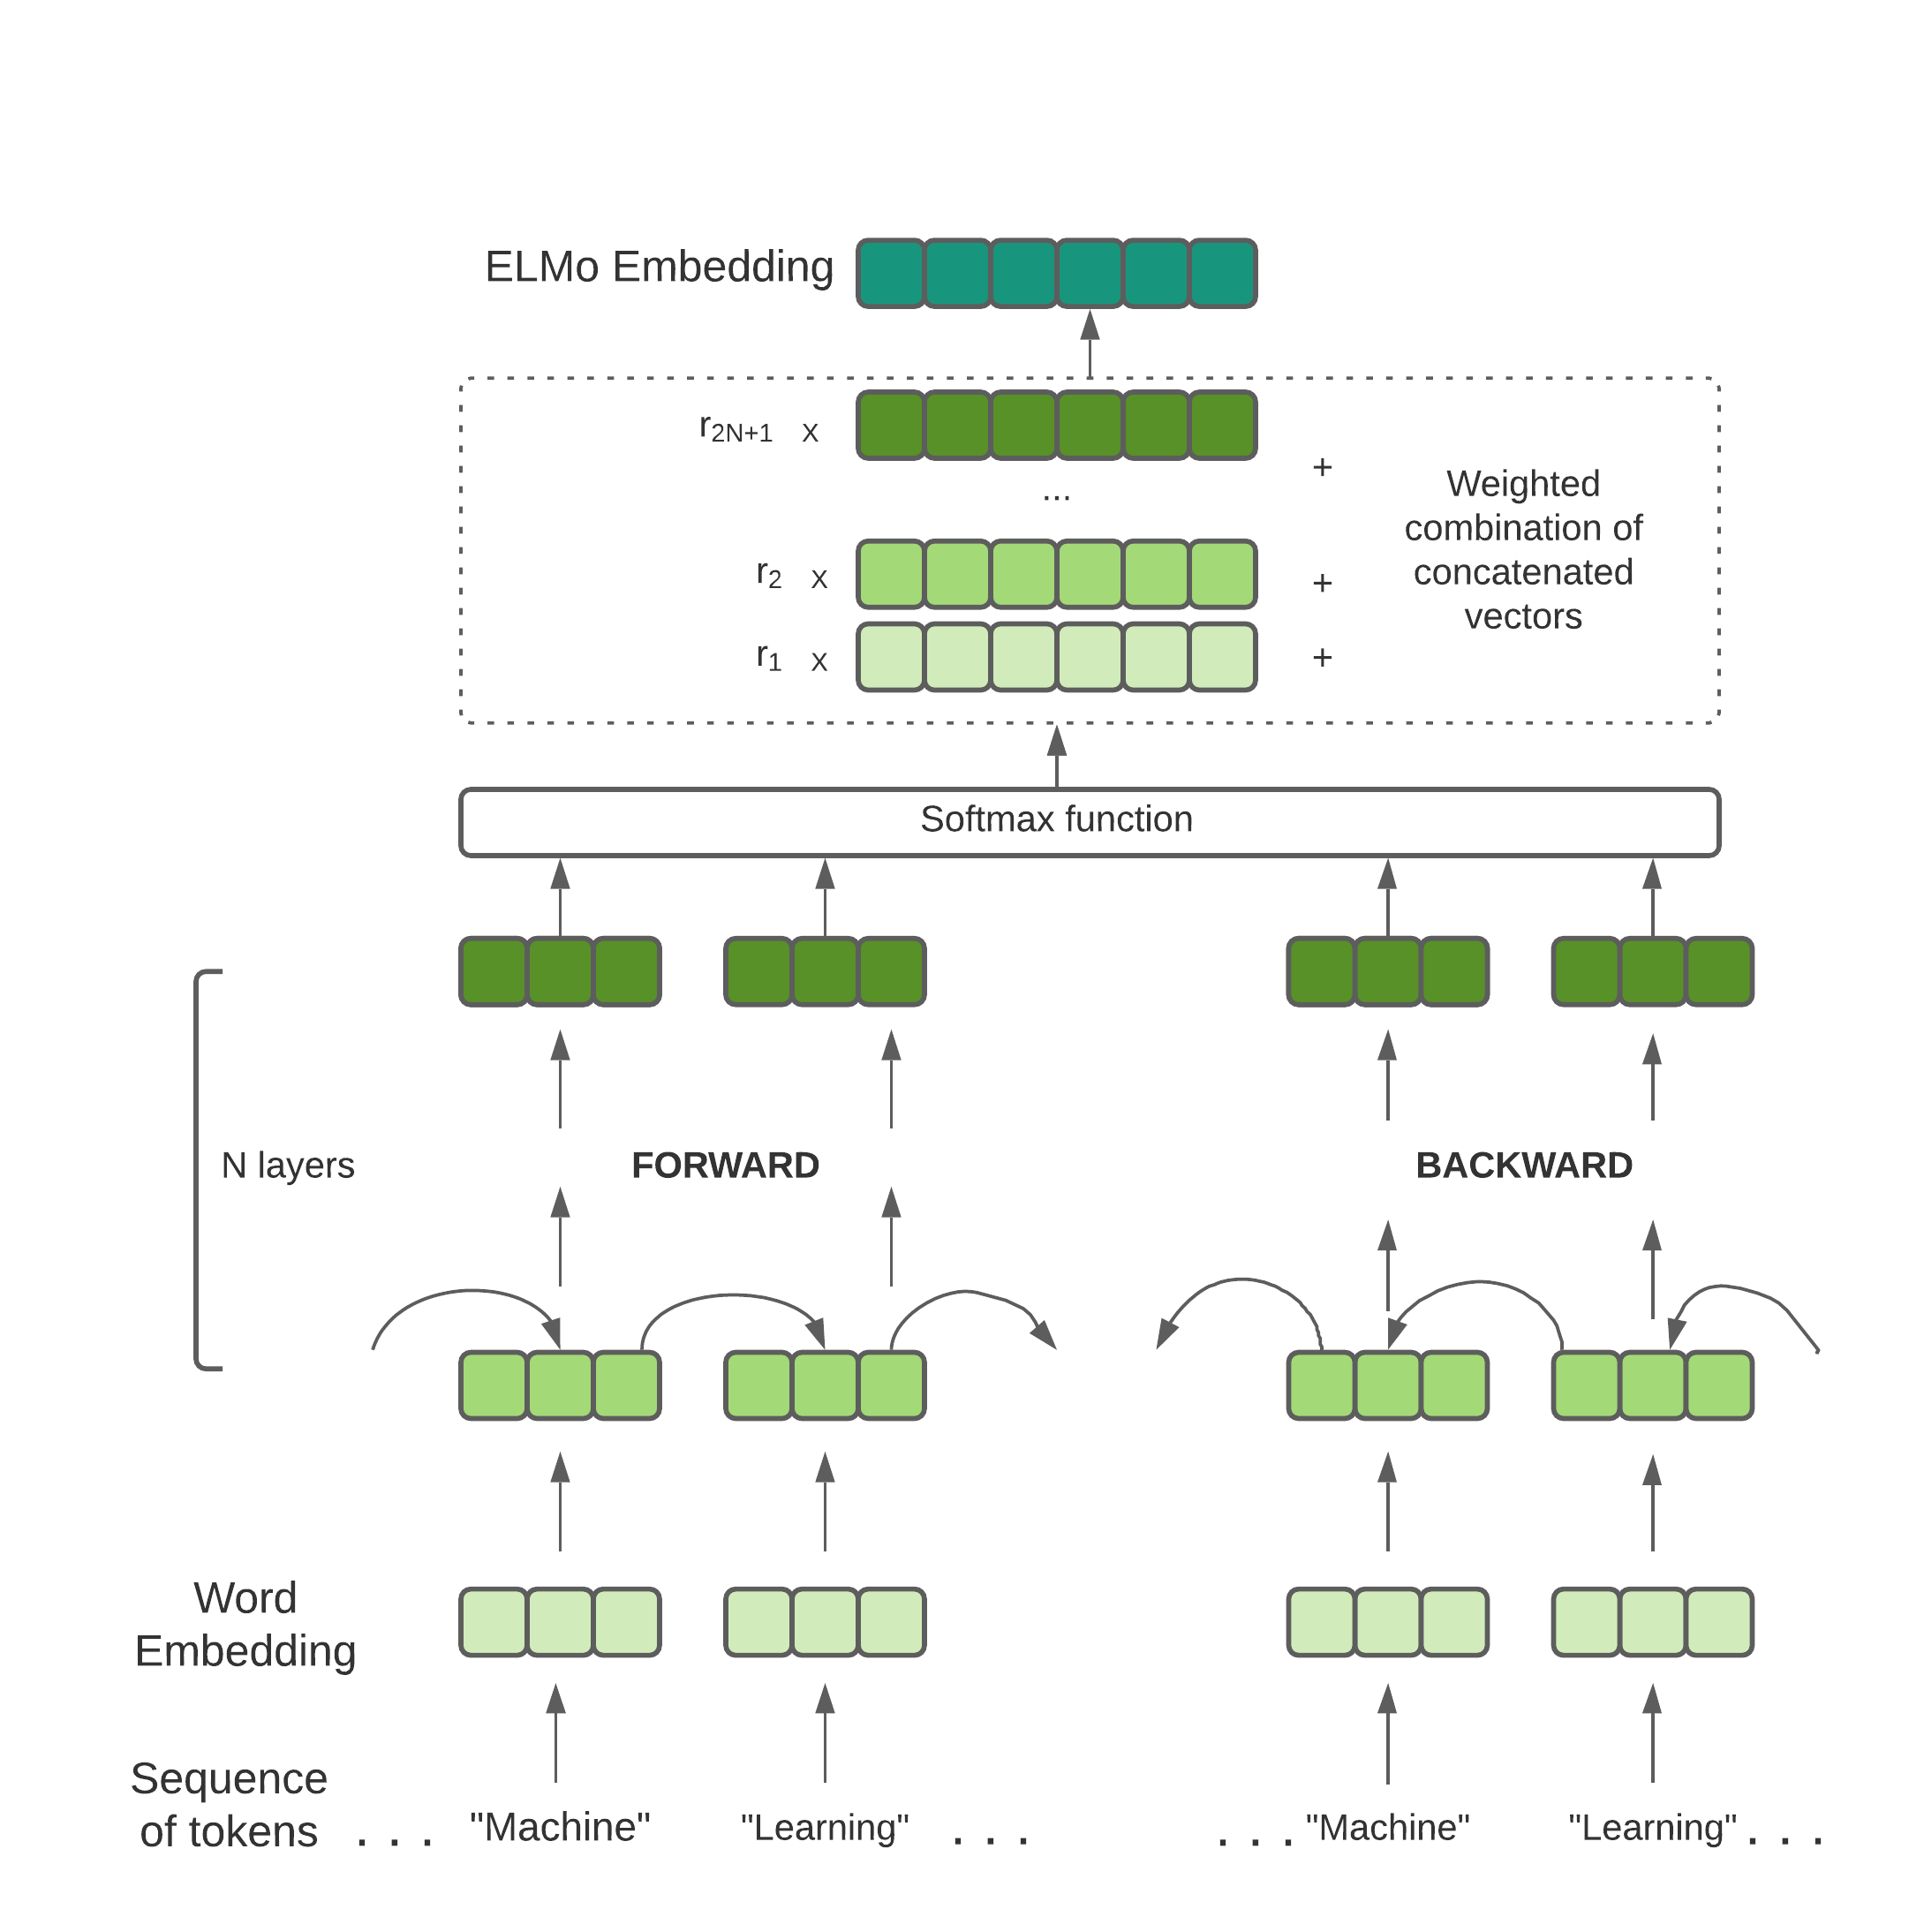
\includegraphics[scale=0.15]{images/Elmo2.png}
\caption{Embeddings from Language Models (ELMo) Context Representation}
\end{figure}


The outline of the ELMo model is as follows:~\cite{context2vec}

\begin{enumerate}
    \item The network consists of N bi-directional (left-to-right and right-to-left) LSTM layers and the input is  a sequence of N words/ tokens. 
    
    \item The Forward language model gets a sequence of words/ tokens (of arbitrary length) from left to right and calculates the probability of the sequence of words  $P(w_1, w_2, ... w_N)$ by making use of the history of words/tokens it has seen earlier~\cite{elmo_word_rep}.
        \begin{center}
            $P(w_1, w_2, ... w_N) = \prod_{i = 1}^{N} P (w_i | w_{1}, w_{2}, w_{i-1})$ 
        \end{center}
        
        For a target word/token $w_i$, let the context-dependent vector from this (forward) language model (at layer l = 1..N) be represented as LRV(i, l), which contains information about this word given the context of words appearing before the target word~\cite{elmo_word_rep}.
        
     \item Similarly, the backward model computes the probability of the reverse sequence of words as follows:
        
        \begin{center}
            $P(w_1, w_2, ... w_N) = \prod_{i = 1}^{N} P (w_i | w_{i+1}, w_{i+2}, w_N)$
        \end{center}
        
        For a target word/token $w_i$, let the context-dependent vector from this (backward) language model (at layer l = 1..N) be represented as RLV(i, l), which contains information about this word given the context of words appearing after the target word~\cite{elmo_word_rep}.
        
        \item The outputs from these models are passed to the subsequent layer of their respective models. A non-linear activation function (for example, ReLU) can be applied for intermediate layers. Softmax is applied to the outputs from the last LSTM layers of the 2 models~\cite{context2vec}.
    
        \item The objective function is to jointly maximise the log-likelihood in both forward and backward directions.
        
        \item For each word $w_i$, a N-layer biLM model will have a total of 2N+1 (including the input sequence of tokens layer) vector representations. The final vector (ELMo) which will be passed to the NLP training model, will combine these 2L+1 vectors by using a weighted sum of these vectors as seen in Figure 3. This is the ELMo embedding~\cite{elmo_word_rep}.
    
\end{enumerate}